\documentclass[11pt]{article}
\usepackage{url}
\usepackage{amsmath, amssymb}
%%%%%%%%%%%%%%%%%%%%%%%%%%%%%%%%%%%%%%%%%
% Cleese Assignment
% Structure Specification File
% Version 1.0 (27/5/2018)
%
% This template originates from:
% http://www.LaTeXTemplates.com
%
% Author:
% Vel (vel@LaTeXTemplates.com)
%
% License:
% CC BY-NC-SA 3.0 (http://creativecommons.org/licenses/by-nc-sa/3.0/)
% 
%%%%%%%%%%%%%%%%%%%%%%%%%%%%%%%%%%%%%%%%%

%----------------------------------------------------------------------------------------
%	PACKAGES AND OTHER DOCUMENT CONFIGURATIONS
%----------------------------------------------------------------------------------------

\usepackage{lastpage} % Required to determine the last page number for the footer

\usepackage{graphicx} % Required to insert images

\setlength\parindent{0pt} % Removes all indentation from paragraphs

\usepackage[most]{tcolorbox} % Required for boxes that split across pages

\usepackage{booktabs} % Required for better horizontal rules in tables

\usepackage{listings} % Required for insertion of code

\usepackage{etoolbox} % Required for if statements

%----------------------------------------------------------------------------------------
%	MARGINS
%----------------------------------------------------------------------------------------

\usepackage{geometry} % Required for adjusting page dimensions and margins

\geometry{
	paper=a4paper, % Change to letterpaper for US letter
	top=3cm, % Top margin
	bottom=3cm, % Bottom margin
	left=2.5cm, % Left margin
	right=2.5cm, % Right margin
	headheight=14pt, % Header height
	footskip=1.4cm, % Space from the bottom margin to the baseline of the footer
	headsep=1.2cm, % Space from the top margin to the baseline of the header
	%showframe, % Uncomment to show how the type block is set on the page
}

%----------------------------------------------------------------------------------------
%	FONT
%----------------------------------------------------------------------------------------

\usepackage[utf8]{inputenc} % Required for inputting international characters
\usepackage[T1]{fontenc} % Output font encoding for international characters

\usepackage[sfdefault,light]{roboto} % Use the Roboto font

%----------------------------------------------------------------------------------------
%	HEADERS AND FOOTERS
%----------------------------------------------------------------------------------------

\usepackage{fancyhdr} % Required for customising headers and footers

\pagestyle{fancy} % Enable custom headers and footers

\lhead{\small\assignmentClass\ifdef{\assignmentClassInstructor}{\ (\assignmentClassInstructor):}{}\ \assignmentTitle} % Left header; output the instructor in brackets if one was set
\chead{} % Centre header
\rhead{\small\ifdef{\assignmentAuthorName}{\assignmentAuthorName}{\ifdef{\assignmentDueDate}{Due\ \assignmentDueDate}{}}} % Right header; output the author name if one was set, otherwise the due date if that was set

\lfoot{} % Left footer
\cfoot{\small Page\ \thepage\ of\ \pageref{LastPage}} % Centre footer
\rfoot{} % Right footer

\renewcommand\headrulewidth{0.5pt} % Thickness of the header rule

%----------------------------------------------------------------------------------------
%	MODIFY SECTION STYLES
%----------------------------------------------------------------------------------------

\usepackage{titlesec} % Required for modifying sections

%------------------------------------------------
% Section

\titleformat
{\section} % Section type being modified
[block] % Shape type, can be: hang, block, display, runin, leftmargin, rightmargin, drop, wrap, frame
{\Large\bfseries} % Format of the whole section
{\assignmentQuestionName~\thesection} % Format of the section label
{6pt} % Space between the title and label
{} % Code before the label

\titlespacing{\section}{0pt}{0.5\baselineskip}{0.5\baselineskip} % Spacing around section titles, the order is: left, before and after

%------------------------------------------------
% Subsection

\titleformat
{\subsection} % Section type being modified
[block] % Shape type, can be: hang, block, display, runin, leftmargin, rightmargin, drop, wrap, frame
{\itshape} % Format of the whole section
{(\alph{subsection})} % Format of the section label
{4pt} % Space between the title and label
{} % Code before the label

\titlespacing{\subsection}{0pt}{0.5\baselineskip}{0.5\baselineskip} % Spacing around section titles, the order is: left, before and after

\renewcommand\thesubsection{(\alph{subsection})}

%----------------------------------------------------------------------------------------
%	CUSTOM QUESTION COMMANDS/ENVIRONMENTS
%----------------------------------------------------------------------------------------

% Environment to be used for each question in the assignment
\newenvironment{question}{
	\vspace{0.5\baselineskip} % Whitespace before the question
	\section{} % Blank section title (e.g. just Question 2)
	\lfoot{\small\itshape\assignmentQuestionName~\thesection~continued on next page\ldots} % Set the left footer to state the question continues on the next page, this is reset to nothing if it doesn't (below)
}{
	\lfoot{} % Reset the left footer to nothing if the current question does not continue on the next page
}

%------------------------------------------------

% Environment for subquestions, takes 1 argument - the name of the section
\newenvironment{subquestion}[1]{
	\subsection{#1}
}{
}

%------------------------------------------------

% Command to print a question sentence
\newcommand{\questiontext}[1]{
	\textbf{#1}
	\vspace{0.5\baselineskip} % Whitespace afterwards
}

%------------------------------------------------

% Command to print a box that breaks across pages with the question answer
\newcommand{\answer}[1]{
	\begin{tcolorbox}[breakable, enhanced]
		#1
	\end{tcolorbox}
}

%------------------------------------------------

% Command to print a box that breaks across pages with the space for a student to answer
\newcommand{\answerbox}[1]{
	\begin{tcolorbox}[breakable, enhanced]
		\vphantom{L}\vspace{\numexpr #1-1\relax\baselineskip} % \vphantom{L} to provide a typesetting strut with a height for the line, \numexpr to subtract user input by 1 to make it 0-based as this command is
	\end{tcolorbox}
}

%------------------------------------------------

% Command to print an assignment section title to split an assignment into major parts
\newcommand{\assignmentSection}[1]{
	{
		\centering % Centre the section title
		\vspace{2\baselineskip} % Whitespace before the entire section title
		
		\rule{0.8\textwidth}{0.5pt} % Horizontal rule
		
		\vspace{0.75\baselineskip} % Whitespace before the section title
		{\LARGE \MakeUppercase{#1}} % Section title, forced to be uppercase
		
		\rule{0.8\textwidth}{0.5pt} % Horizontal rule
		
		\vspace{\baselineskip} % Whitespace after the entire section title
	}
}

%----------------------------------------------------------------------------------------
%	TITLE PAGE
%----------------------------------------------------------------------------------------

\author{\textbf{\assignmentAuthorName}} % Set the default title page author field
\date{} % Don't use the default title page date field

\title{
	\thispagestyle{empty} % Suppress headers and footers
	\vspace{0.2\textheight} % Whitespace before the title
	\textbf{\assignmentClass:\ \assignmentTitle}\\[-4pt]
	\ifdef{\assignmentDueDate}{{\small Due\ on\ \assignmentDueDate}\\}{} % If a due date is supplied, output it
	\ifdef{\assignmentClassInstructor}{{\large \textit{\assignmentClassInstructor}}}{} % If an instructor is supplied, output it
	\vspace{0.32\textheight} % Whitespace before the author name
}
 % Include the file specifying the document structure and custom commands

%----------------------------------------------------------------------------------------
%	ASSIGNMENT INFORMATION
%----------------------------------------------------------------------------------------

% Required
\newcommand{\assignmentQuestionName}{Question} % The word to be used as a prefix to question numbers; example alternatives: Problem, Exercise
\newcommand{\assignmentClass}{EE498} % Course/class
\newcommand{\assignmentTitle}{HW 6} % Assignment title or name
\newcommand{\assignmentAuthorName}{Muhammed İzzet Sezer} % Student name

% Optional (comment lines to remove)
\newcommand{\assignmentClassInstructor}{Klaus Werner Schmidt} % Intructor name/time/description
\newcommand{\assignmentDueDate}{07\ 06,\ 2023} % Due date

%----------------------------------------------------------------------------------------

\begin{document}

%----------------------------------------------------------------------------------------
%	TITLE PAGE
%----------------------------------------------------------------------------------------

\maketitle % Print the title page

\thispagestyle{empty} % Suppress headers and footers on the title page

\newpage

\paragraph*{Project Link:} \url{https://github.com/sezer-muhammed/EE408-HW6}

\begin{question}

	\questiontext{Simulation and Analysis}

	\begin{subquestion}{Write down the process regulation for the given Butcher Tableau}

	\end{subquestion}
	\answer{
		\begin{enumerate}
			\item Compute the first slope, $k_1$, using the formula: $k_1 = h f(t_i, y_i)$.
			\item Next, calculate $k_2$, which uses the midpoint of the interval for function value approximation. The formula is: $k_2 = h f(t_i + c_2 h, y_i + c_2 k_1)$.
			\item Determine $k_3$ via the formula: $k_3 = h f(t_i + 2 c_2 h, y_i + c_2 k_2)$. This approximates the slope at the midpoint of the interval using the second stage's value.
			\item Lastly, find the approximation of the solution at the next step, $y_{i+1}$, using the formula: $y_{i+1} = y_i + \frac{1}{3} (k_1 + k_2 + k_3)$.
		\end{enumerate}

		$f(t, y)$ is the function that describes the differential equation, $h$ is the size of the step, $(t_i, y_i)$ represent the current time and function value, respectively, and $c_2$ is a pre-specified constant.


	}

	\begin{subquestion}{Perform the local error}

	\end{subquestion}
	\answer{
	\begin{equation}
	y(t_{i+1}) = y(t_i) + h f(t_i, y_i) + \frac{h^2}{2} f'(t_i, y_i) + \frac{h^3}{6} f''(t_i, y_i) + O(h^4),
	\end{equation}
	The three-stage Runge-Kutta method, whose expansions are:
	
	\begin{align*}
	k_1 &= h f(t_i, y_i), \\
	k_2 &= h f(t_i + c_2 h, y_i + c_2 k_1) = h f(t_i, y_i) + c_2 h^2 f'(t_i, y_i) + O(h^3), \\
	k_3 &= h f(t_i + 2 c_2 h, y_i + c_2 k_2) = h f(t_i, y_i) + 2 c_2 h^2 f'(t_i, y_i) + O(h^3), \\
	y_{i+1} &= y_i + k_1 \cdot 0 + k_2 \cdot 0 + k_3 \cdot 1 = y_i + h f(t_i, y_i) + 2 c_2 h^2 f'(t_i, y_i) + O(h^3). \\
	\end{align*}
	
	1- The initial term (up to $h$ order) in both series is identical for all $c_2$ values. Therefore, irrespective of the $c_2$ value, the method displays a first order ($p=1$) accuracy.

	2- However, achieving second-order ($p=2$) accuracy requires the $h^2$ terms of the series to match. This occurs exclusively when $c_2$ equals $\frac{1}{4}$, as shown by the Runge-Kutta method expansion. Therefore, $c_2 = \frac{1}{4}$ is the unique condition under which the method reaches a second-order accuracy.
	}

	\begin{subquestion}{Determine the region of stability for the suggested Runge-Kutta method}

	\end{subquestion}
	\answer{

	The region of stability (ROS) is a crucial concept in the context of numerical solutions for differential equations. It represents the set of complex numbers $\zeta = h \lambda$, where $h$ is the numerical method's step size and $\lambda$ is the eigenvalue of the system under consideration, which allows for a stable solution.

	The notion of stability, in this context, relates to the behavior of solutions over time. For a stable method applied to the linear differential equation $y' = \lambda y$, the solutions do not increase in absolute value as time goes on.
	
	Given our particular Butcher tableau (with $c_2 = 1/4$), we can determine the stability function (or amplification factor) for this Runge-Kutta method as:
	
	\begin{equation}
		R(\sigma ) = 1 + \sigma + \frac{\sigma^2}{2},
		\end{equation}
		
	
	with $\sigma = h \lambda$. The ROS is then characterized by the subset of the complex plane for which the absolute value of the stability function does not exceed 1. Formally, this can be written as:
	
	\begin{equation}
		\{ \sigma \in {C} : |R(\sigma)| \leq 1 \}.
		\end{equation}
		
	
	This subset gives us all possible values of $\zeta=h\lambda$ that ensure the stability of our numerical method. By plotting this region, we can better understand the method's efficacy across different problems, which can be defined by diverse $\lambda$ values and various step sizes $h$.
	
	In the following figures, we show the boundary of the ROS, indicating the points for which the absolute value of the stability function equals 1. Also, we illustrate how the ROS changes with different step sizes.
	\begin{center}
		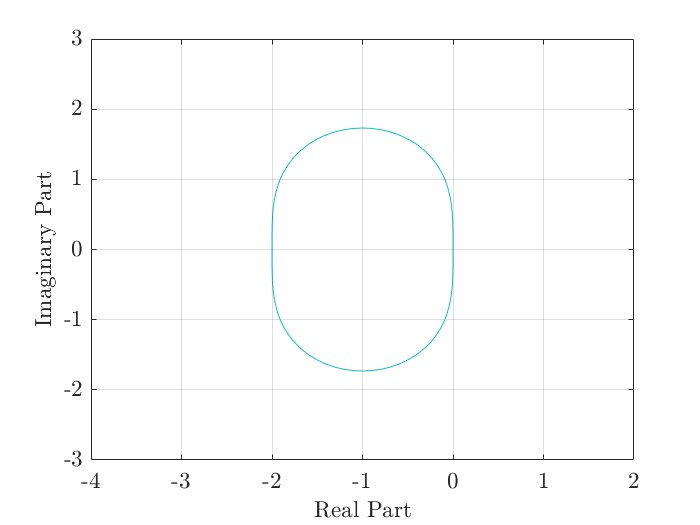
\includegraphics[width=0.7\columnwidth]{1.jpg} % Example image
	\end{center}
	\begin{center}
		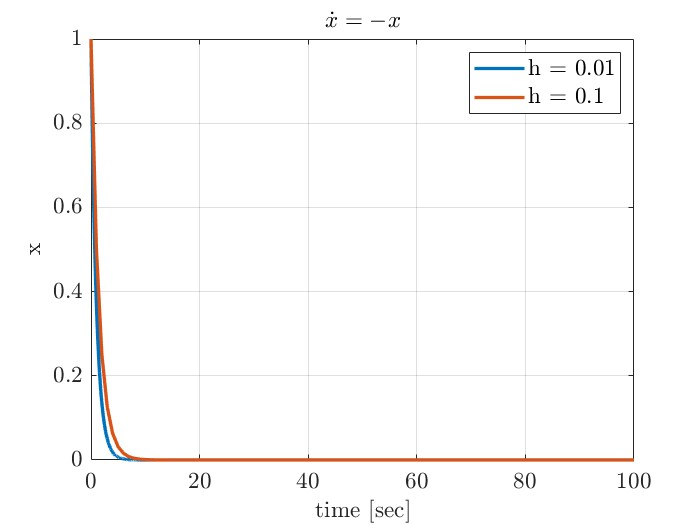
\includegraphics[width=0.7\columnwidth]{2.jpg} % Example image
	\end{center}
	
	}

	\begin{subquestion}{Analyze why the method becomes instable for h > 1.25 for the linear system}

	\end{subquestion}
	\answer{
		In the case of the linear system $\dot{x} = -5x$, the system's eigenvalue is $\lambda = -5$. When this eigenvalue is introduced into the Runge-Kutta stability function, we find that the stability condition becomes:

		\begin{equation}
		|1 + h\lambda + \frac{(h\lambda)^2}{2}| \leq 1
		\end{equation}
		
		For this system, this condition simplifies to:
		
		\begin{equation}
		|1 - 5h + 12.5h^2| \leq 1
		\end{equation}
		
		The method is stable when the absolute value of this expression is less than or equal to 1. If $h > 1.25$, the absolute value of the expression exceeds 1, and the method becomes unstable.
		
		The reason for this instability is that the step size $h$ becomes too large relative to the system's eigenvalue $\lambda$. The quantity $h\lambda = -5h$ is a measure of the total change in $x$ over a single step. If this quantity is too large (in absolute value), then the method's estimate of $x$ at the next step will overshoot the true value, leading to instability.
		
		To determine for which values of $h$ the resulting $\sigma = h\lambda$ lies in the ROS, we can substitute $\sigma = h\lambda$ into the stability condition and solve for $h$:
		
		\begin{equation}
		|1 + \sigma + \frac{\sigma^2}{2}| \leq 1
		\end{equation}
		
		This yields:
		
		\begin{equation}
		|1 - 5h + 12.5h^2| \leq 1
		\end{equation}
		
		Solving this inequality for $h$, we find that the method is stable for $-1.25 \leq h \leq 1.25$. These are the values of $h$ for which $\sigma = h\lambda$ lies in the ROS. If $h > 1.25$, the method becomes unstable because $\sigma$ falls outside the ROS.

	}

\end{question}


\end{document}
